
\section{Residuals and Diagnostics}

* For a given value X of the independent variable, the value predicted by regression line $\hat{y}$ is often called the \textbf{fitted
value} of the dependent variable. 
* The difference between the observed value Y and the fitted value Y
is called the residual for that observation and is denoted by \textbf{e}:
\[e= Y-\hat{Y}\]

* (Important for later: Residuals represent unexplained (or residual) variation after fitting a regression
model. )
For the example used in this class, the residuals are very small.

%%%%%%%%%%%%%%%%%%%%%%%%%%%%%%%%%%%%%%%%%%%%%

\begin{figure}
\centering
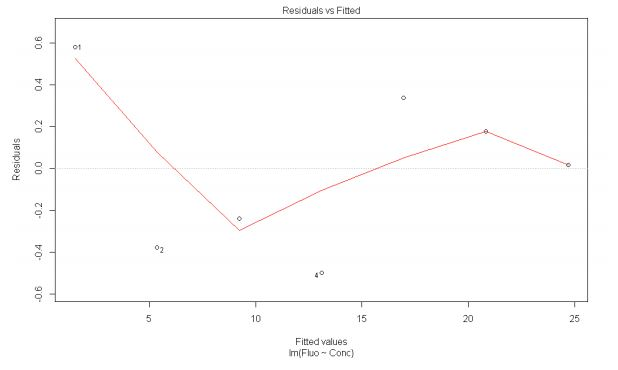
\includegraphics[width=1.1\linewidth]{ResidPlot1}
\end{figure}

#### Normality of Residuals
Additionally, the linear model approach requires this assumption that the residuals are normally
distributed. We can use a Q-Q plot to assess the normality of residuals.
\begin{figure}
\centering
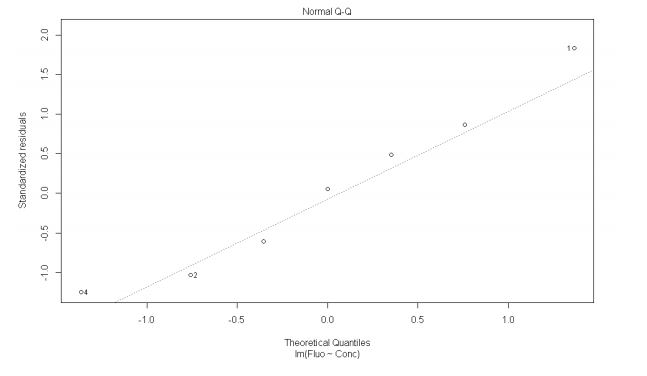
\includegraphics[width=1.1\linewidth]{ResidPlot2}
\end{figure}



av plots Cook's D plot influence plot click to view
%=== %
#### Non-normality}

```{r}
# Normality of Residuals
# qq plot for studentized resid
qqPlot(fit, main="QQ Plot")

# distribution of studentized residuals
library(MASS)
sresid <- studres(fit) 
hist(sresid, freq=FALSE, 
main="Distribution of Studentized Residuals")
xfit<-seq(min(sresid),max(sresid),length=40) 
yfit<-dnorm(xfit) 
lines(xfit, yfit)


qq plot histogram of studentized residuals click to view
%= %
\section{Non-constant Error Variance}

Evaluate homoscedasticity

```{r}
# non-constant error variance test
ncvTest(fit)
# plot studentized residuals vs. fitted values 
spreadLevelPlot(fit)
spread vs. levels click to view


%= %
Multi-collinearity

```{r}
# Evaluate Collinearity
vif(fit) # variance inflation factors 
sqrt(vif(fit)) > 2 # problem?


%==== %
#### Nonlinearity}

```{r}
# Evaluate Nonlinearity
# component + residual plot 
crPlots(fit)
# Ceres plots 
ceresPlots(fit)


component plus residual plot Ceres plots click to view
%== %
\section{Non-independence of Errors}

The Durbin–Watson statistic is a test statistic used to detect the presence of autocorrelation (a relationship between values separated from each other by a given time lag) in the residuals (prediction errors) from a regression analysis. It is named after James Durbin and Geoffrey Watson.

```{r}
# Test for Autocorrelated Errors
durbinWatsonTest(fit)


\end{document}

# Assessing Outliers
outlierTest(FitAll) # Bonferonni p-value for most extreme obs
qqPlot(FitAll, main="QQ Plot") #qq plot for studentized resid 
leveragePlots(FitAll) # leverage plots
leverage plot click to view
Influential Observations
# Influential Observations
# added variable plots 
av.Plots(FitAll)
# Cook's D plot
# identify D values > 4/(n-k-1) 
cutoff <- 4/((nrow(mtcars)-length(FitAll$coefficients)-2)) 
plot(FitAll, which=4, cook.levels=cutoff)
# Influence Plot 
influencePlot(FitAll,id.method="identify", main="Influence Plot", sub="Circle size is proportial to Cook's Distance" )
av plots Cook's D plot influence plot click to view
Non-normality
# Normality of Residuals
# qq plot for studentized resid
qqPlot(FitAll, main="QQ Plot")
# distribution of studentized residuals
library(MASS)
sresid <- studres(FitAll) 
hist(sresid, freq=FALSE, 
main="Distribution of Studentized Residuals")
xFitAll<-seq(min(sresid),max(sresid),length=40) 
yFitAll<-dnorm(xFitAll) 
lines(xFitAll, yFitAll)
qq plot histogram of studentized residuals click to view
Non-constant Error Variance
# Evaluate homoscedasticity
# non-constant error variance test
ncvTest(FitAll)
# plot studentized residuals vs. FitAllted values 
spreadLevelPlot(FitAll)
spread vs. levels click to view
Multi-collinearity
# Evaluate Collinearity
vif(FitAll) # variance inflation factors 
sqrt(vif(FitAll)) > 2 # problem?
Nonlinearity
# Evaluate Nonlinearity
# component + residual plot 
crPlots(FitAll)
# Ceres plots 
ceresPlots(FitAll)
component plus residual plot Ceres plots click to view
Non-independence of Errors
# Test for Autocorrelated Errors
durbinWatsonTest(FitAll)
